\documentclass{article}
\usepackage[utf8]{inputenc}

\title{WydenArea1AlgoritmoComputacional}
%\author{Heleno Cardoso}
\author{
  Heleno Cardoso da S. Filho\thanks{PPGCOMP UNIFACS - Mestre em Sistemas e Computação -- PGCOMP UFBA [Aluno Especial no Doutorado em Ciência da Computação].} \\
  Departamento de Engenharia\\
  Wyden Faculdade Área 1\\
  Brasil - Adtalem Global Education\\
  \texttt{helenocardosofilho@gmail.com} \\
  %% examples of more authors
  %% \And
  %% Coauthor \\
  %% Affiliation \\
  %% Address \\
  %% \texttt{email} \\
  %% \AND \\
}

\date{August 2018}

\usepackage{natbib}
\usepackage{graphicx}
\usepackage{verbatim}

\begin{document}

\maketitle

\section{Disciplina Algoritmo Computacional - Wyden Área 1}

% Operação com Binários: http://www.multicalculadora.com.br/

Algoritmo é uma sequência finita de instruções bem definidas e não ambíguas, cada uma das quais devendo ser executadas mecânica ou eletronicamente em um intervalo de tempo finito e com uma quantidade de esforço finita. \\

A cada dia torna-se mais notável a participação da máquina no auxílio de tarefas humanas. Em destaque, o computador (PC) se faz cada vez mais presente nos lares e, principalmente, em empresas, indo da micro até a algumas grandes empresas que não sentem a necessidade de um computador "especial". O grande sucesso do PC se deu por vários fatores, como: baixo custo, compatibilidade de recursos internos e externos (exemplo interno: o barramento PCI; externo: os dispositivos USB) entre outros fatores. Porém pode-se dizer que os principais fatores, entre todos os outros, são a grande quantidade de programas disponíveis e a fácil utilização destes. \\

Aqui vamos falar sobre os algoritmos computacionais que podemos chamar de o b-a-bá das linguagens de programação1. Utilizaremos inicialmente uma linguagem conhecida por pseudo-linguagem, que é uma linguagem fictícia, ou seja, os principais comandos de programação escritos em português de forma fácil de entender. Após, utilizaremos a linguagem C2 como ferramenta para nossos estudos. 

\begin{figure}[h!]
\centering
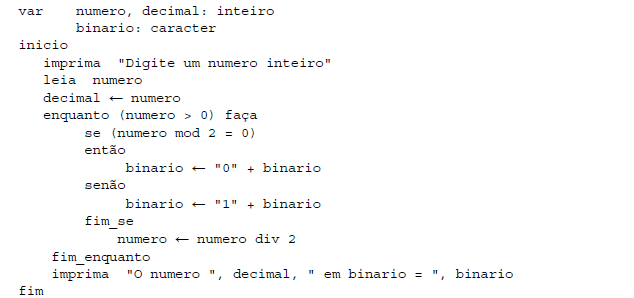
\includegraphics[scale=0.9]{FigAlgoritmoComputacional}
\caption{Algoritmo Computacional}
\label{fig:AlgoritmoComputacional}
\end{figure}

\section{Conheça o nosso curso de Lógica de Programação Completo.
Linguagens de alto nível}

Com a popularidade dos computadores criou-se um “problema”: alta demanda por software e, consequentemente, por programadores. Talvez você esteja pensando que isso não é exatamente um problema, e sim uma coisa boa, uma tendência, um novo mercado. Faz sentido, até certo ponto. O problema era encontrar mão de obra qualificada para codificar àquelas instruções tão complicadas.

Com isso, novas linguagens surgiram e, cada vez mais, aproximavam-se da linguagem humana. Isso abriu “fronteiras” para que uma enorme gama de novos desenvolvedores se especializassem. Tais linguagens são denominadas como sendo de alto nível. As linguagens modernas que hoje conhecemos e usamos são de alto nível: C, PHP, Java, Rust, C\#, Python, Ruby etc.

Quanto mais próxima da linguagem da máquina, mais baixo nível é a linguagem. Quanto mais próxima da linguagem humana, mais alto nível ela é.

Paradigmas das linguagens de programação
Quando uma linguagem de programação é criada, a partir das suas características, ela é categorizada em um ou mais paradigmas.

A definição do dicionário Aurélio para “paradigma”:

Algo que serve de exemplo geral ou de modelo.
Conjunto das formas que servem de modelo de derivação ou de flexão.
Conjunto dos termos ou elementos que podem ocorrer na mesma posição ou contexto de uma estrutura.
O paradigma de uma linguagem de programação é a sua identidade. Corresponde a um conjunto de características que, juntas, definem como ela opera e resolve os problemas. Algumas linguagens, inclusive, possuem mais de um paradigma, são as chamadas multi paradigmas.

Alguns dos principais paradigmas utilizados hoje no mercado:

\begin{enumerate}
    \item  Funcional
    \item  Lógico
    \item  Declarativo
    \item  Imperativo
    \item  Orientado a objetos
    \item  Orientado a eventos
\end{enumerate}

Paradigma funcional
O foco desse paradigma está na avaliação de funções. Como na matemática quando temos, por exemplo, uma função f(x):

f(x) = x + 2
x é um parâmetro (o valor de entrada) e, após a expressão ser avaliada, obtêm-se o resultado.

Se o valor de entrada for 2, o resultado da avaliação da nossa função será 4.

Algumas das linguagens que atendem a esse paradigma: F\# (da Microsoft), Lisp, Heskell, Erlang, Elixir, Mathematica.

É possível desenvolver de forma “funcional” mesmo em linguagens não estritamente funcionais. Por exemplo, no PHP, que é uma linguagem multi paradigma, teríamos:

<?php

 \begin{comment}
$sum = function($value) {
    return $value + 2;
};
echo $sum(2); // 4
 \end{comment}

Paradigma lógico
Também é conhecido como “restritivo”. Muito utilizado em aplicações de inteligência artificial. Esse paradigma chega no resultado esperado a partir de avaliações lógico-matemáticas. Se você já estudou lógica de predicados, confortável se sentirá em entender como uma linguagem nesse paradigma opera.

Principais elementos desse paradigma:

Proposições: base de fatos concretos e conhecidos.
Regras de inferência: definem como deduzir proposições.
Busca: estratégias para controle das inferências.
Exemplo:

Proposição: Chico é um gato.
Regra de inferência: Todo gato é um felino.
Busca: Chico é um felino?
A resposta para a Busca acima precisa ser verdadeira. A conclusão lógica é:

Se Chico é um gato e todo gato é felino, então Chico é um felino.

A idéia básica da programação em lógica é:

“Oferecer um arcabouço que permita inferir conclusões desejadas, a partir de premissas, representando o conhecimento disponível, de uma forma que seja computacionalmente viável”. Prof. Dr. Silvio do Lago Pereira – DTI / FATEC-SP.

A linguagem mais conhecida que utiliza esse paradigma é a Prolog. Esse paradigma é pouco utilizado em aplicações comerciais, seu uso se dá mais na área acadêmica.

Leitura recomendada: https://www.ime.usp.br/~slago/pl-1.pdf

Paradigma declarativo
O paradigma declarativo é baseado no lógico e funcional. Linguagens declarativas descrevem o que fazem e não exatamente como suas instruções funcionam.

Linguagens de marcação são o melhor exemplo: HTML, XML, XSLT, XAML etc. Não obstante, o próprio Prolog – reconhecido primariamente pelo paradigma lógico – também é uma linguagem declarativa. Abaixo alguns exemplos dessas linguagens.

HTML:

<article>
  <header>
    <h1>Linguagens e paradigmas de programação</h1>
  </header>
</article>
SQL:

SELECT nome FROM usuario WHERE id = 10

Paradigma imperativo
Você já ouviu falar em “programação procedural” ou em “programação modular“? De modo geral, são imperativas.

Linguagens clássicas como C, C++, PHP, Perl, C\#, Ruby etc, “suportam” esse paradigma. Ele é focado na mudança de estados de variáveis (ao contrário dos anteriores).

Exemplo:

if(option == 'A') {
    print("Opção 'A' selecionada.");
}
A impressão só será realizada se o valor da variável option for igual a A.

Paradigma orientado a objetos
Esse é, entre todos, talvez o mais difundido. Nesse paradigma, ao invés de construirmos nossos sistemas com um conjunto estrito de procedimentos, assim como se faz em linguagens “fortemente imperativas” como o Cobol, Pascal etc, na orientação a objetos utilizamos uma lógica bem próxima do mundo real, lidando com objetos, estruturas que já conhecemos e sobre as quais possuímos uma grande compreensão.

OO é sigla para orientação a objetos

O paradigma orientado a objetos tem uma grande preocupação em esconder o que não é importante e em realçar o que é importante. Nele, implementa-se um conjunto de classes que definem objetos. Cada classe determina o comportamento (definido nos métodos) e estados possíveis (atributos) de seus objetos, assim como o relacionamento entre eles.

Esse é o paradigma mais utilizado em aplicações comerciais e as principais linguagens o implementam: C\#, Java, PHP, Ruby, C++, Python etc.

Paradigma orientado a eventos
Toda linguagem que faz uso de interface gráfica é baseada nesse paradigma. Nele, o fluxo de execução do software é baseado na ocorrência de eventos externos, normalmente disparados pelo usuário.

\section{Conclusão}

Um algoritmo é caracterizado por qualquer forma de resolver um problema de forma procedural a partir de padrões e regras. Veja um exemplo: \\

Cinco vezes cinco é igual ao número cinco somado cinco vezes. \\

5 X 5 = 5 + 5 + 5 + 5 + 5 \\

Isso, de forma simples, é um algoritmo. \\

O algoritmo computacional se extende dessa idéia. É um programa que realiza procedimentos para solucionar um problema. \\

A diferença está na forma que isso deve ser feito. Algoritmos computacionais usam estruturas que ajudam o processador a chegar a um determinado resultado. Ou seja, o programador tem que realmente expressar como chegar ao resultado passo-a-passo, pois não existe o óbvio para o computador.

Para isso, define-se que para criar um algoritmo (programa) é apenas necessário três estruturas:

Estrutura de procedimento

Estrutura seletiva

Estrutura repetitiva

E, para isso, podemos também usar alguns paradigmas dos dias atuais, como a programação orientada a eventos e a programação orientada a objetos.

\bibliographystyle{plain}
\bibliography{references}
\end{document}
